%!TEX root = main_thesis.tex
%---------------------------------------------------------------------------------
\chapter{A CFO Estimation Method for OFDM Synchronisation}
\label{chap:CFO}
%---------------------------------------------------------------------------------

%---------------------------------------------------------------------------------
\section{Introduction}
%---------------------------------------------------------------------------------
In the previous chapter, robust OFDM timing synchronisation was explored, leading to a proposed method that is able to perform well even in the case of large fractional CFO.
However, the CFO estimation of that method was only estimate the fractional CFO rather than large integer CFO that can occur as a result of the Doppler Effect and/or due to local oscillator instabilities.
CFO is usually normalised by subcarrier spacing and divided into an integer frequency offset (IFO) part, which is a whole multiple of subcarrier spacings, and a remainder which is referred to as fractional frequency offset (FFO).
IFO causes a circular shift of the subcarrier in the frequency domain while FFO results in ICI because of lost orthogonality between subcarriers.
\begin{figure}[b]
    \centerline{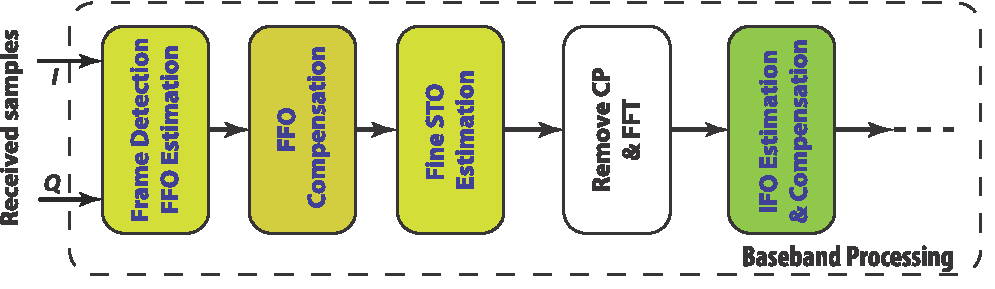
\includegraphics [width=0.9\columnwidth] {figures/Baseband.pdf} }
    \caption{Baseband processing block diagram.}
    \label{fig:baseband}
\end{figure}
Fig.~\ref{fig:baseband} illustrates the process of FFO and IFO estimation in the baseband processing of a typical OFDM system.
The IFO estimation is performed after the FFT, and relies upon cross-correlation, which consumes significant hardware resources.
A typical OFDM receiver avoids the need for IFO estimation by limiting CFO tolerance to be smaller than the range of allowable FFO estimation, resulting in a set of very strict constraints on the design of the RF front-end. However, if CFO exceeds the range of FFO estimation, IFO is present and the system cannot therefore function correctly.
This is more pronounced in applications that subject the front-end to intensive Doppler (including rapidly mobile systems), for very high carrier frequencies, or systems which aim to support multiple frequency bands for different standards.

In this chapter, a novel method is proposed for IFO estimation to overcome this challenge to efficient and low-power implementation. The basis of this method has also been discussed in:
\begin{itemize}
\item T. H. Pham, S. A. Fahmy, and I. V. McLoughlin, ``Efficient Integer Frequency Offset Estimation Architecture for Enhanced OFDM Synchronization,'' to be submitted to \textit{IEEE Transactions on Very Large Scale Integration (VLSI) Systems}.
\end{itemize}

%---------------------------------------------------------------------------------
\section{Related Work}
%---------------------------------------------------------------------------------
As mentioned in the previous chapter, the estimation range of  fractional CFO has a limitation that is shown in (\ref{fractionalCFOlimitation}); for instance its range is up to $\pm$2 sub-carrier spacings in the case of the IEEE~802.16 preamble. The value of the IFO is a multiple of the coarse CFO's range.
It is commonly estimated by performing cross-correlation \cite{Bang2001,Kim2008} in the frequency domain.

Let us assume that the signal is transmitted over a frequency selective channel that has channel impulse response (CIR) $h$ with length, \emph{L} ($L<N_{CP}$), and which is corrupted by AWGN.
The received signal, suffering frequency and timing offsets, can be expressed in the time domain as
\begin{equation}
\label{xnfull}
y[n] = \sum_{l=0}^{L-1} h[l]x[n-\tau-l] e^{i(2\pi \xi \frac{n-\tau}{N} + \phi_0)} + w[n]
\end{equation}
where $w[n]$ denotes AWGN in the time domain, $\tau$, $\phi_0$ are residual timing offset (RTO) and error phase, respectively, and $\xi$ is the normalised CFO that can be divided into an FFO part $\lambda$ and an IFO part $\epsilon$ as $\xi=\lambda+\epsilon$.

Assuming FFO and STO be compensated by earlier stages of synchronisation, as has been investigated in detail by other authors \cite{Kim2008,Pham2014}, the received preamble symbol after CP removal at FFT output is
\begin{equation}
\label{xnrec}
Y[k] =  e^{i(\phi_0-2\pi \frac{\tau k}{N})} H[k-\epsilon] X[k-\epsilon] + W[k]
\end{equation}
where $W[k]$ and $H[k]$ are the frequency domain representations of AWGN and CIR, respectively.
%\todo[inline]{**Thinh: I think it should that $W[k]$ in the above equation (ivm)}

As mentioned previously, IFO results in a cyclic shift in the frequency domain and is commonly estimated by performing cross-correlation in the frequency domain.
By contrast, RTO causes a linear phase rotation on samples in the frequency domain that may cause degradation of cross-correlation performance during IFO estimation.
Based on a differential demodulation of the FFT output, the IFO can be determined with better robustness to frequency selective channel and RTO effects using the correlation function \cite{Park2002} expressed by:

\begin{equation}
\label{integerCFO}
\hat{\epsilon} =\underset{\tilde{\epsilon}}{\operatorname{argmax}}  \left|\sum_{k=1}^{N} Y^{*}[k-1] Y[k]  X^{*}[k-\tilde{\epsilon}]  X[k-1-\tilde{\epsilon}]\right|
\end{equation}
where $(.)^{*}$ denotes complex conjugation, $\hat{\epsilon}$, $\tilde{\epsilon}$ are estimated and trial values of $\epsilon$, respectively,
$Y[k]$ and $X[k]$ denote the $k^{th}$ frequency symbol index of the received symbol and the known transmitted preamble, respectively, and the symbol size $N$ is equal to the FFT size.

The estimated IFO can achieve high precision using cross-correlation in the frequency domain, however implementing cross-correlation clearly involves a significant hardware overhead, with a multiplier needed for each element in the cross-correlation.
Sign-bit cross-correlation \cite{Schwoerer2002} is a widely adopted approach to reducing correlation complexity using only the most significant bit (MSB) of the signed two's complement numbers in the correlation computation. In this way, complexity is reduced at the cost of some performance degradation.
Despite the adoption of such methods, cross-correlation remains computationally expensive, especially when dealing with a large FFT size.
It should be noted here that several IFO estimation methods have been published which claim robustness to frequency selective channels and RTO. However, published FPGA implementations of these methods are lacking to date, possibly because the hardware costs are considerable -- even when adopting the sign-bit cross-correlation approach as mentioned.%}

There are few practical implementations for IFO estimation and correction.
A notable exception was presented in \cite{Kim2008}, in which time-domain cross correlation is performed between received samples and several pre-rotated versions of the preamble corresponding to possible IFO values. Although this method uses efficient sign-bit correlation to reduce hardware cost (at the cost of decreased estimation accuracy and increased sensitive to frequency
selective channels), it is not efficient when the possible IFO range is large since it effectively performs an exhaustive search of possibilities.

State of the art OFDM synchronisation methods typically have a small tolerance of CFO that requires the hardware be strictly constrained to ensure operation within a small CFO range which does not include any IFO.
This strict timing requirement leads to an increase in total system cost. Particularly, in the case of MSCR, the need for high precision timing, coupled with a requirement for a wide ranging and agile operating frequency span, would make the RF front-end design extremely difficult, if not impossible.

%---------------------------------------------------------------------------------
\section{Enhanced OFDM Synchronization Through Novel IFO Estimation Architecture}
%---------------------------------------------------------------------------------
In this section, we propose a novel method in which hardware resources and power consumption are reduced by determining IFO estimates for only a subset of possible IFO values. This in turn enables an efficient resource sharing folded architecture to be adopted. Adjusting the precision of individual correlation computations within this novel architecture leads to a fine degree of control on the trade-off between performance and power consumption.
The implementation uses the long preamble of IEEE~802.16-2009~\cite{IEEE80216} for estimating IFO values.
This preamble has a symbol size of 256 with 100 pilots, as illustrated in Fig.~\ref{fig:long_pre}.
These 100 pilots are distributed, 50 pilots per side, at even sub-carrier spacings from 2 to 100 and from 156 to 254. The remaining sub-carriers are null.
\begin{figure}[b]
    \centerline{\includegraphics [width=1\columnwidth] {figures/long_pre.pdf} }
    \caption{Pilots in the long preamble of IEEE~802.16-2009.}
    \label{fig:long_pre}
\end{figure}
In OFDM-based systems such as 802.11, 802.16, and 802.22, the short preamble is used to estimate and compensate for FFO.
Typically, fractional CFO estimation has a limited range of up to ${\pm}2$ sub-carrier spacings depending on the format of the short preamble.
This results in the possible IFO values being a multiple of 4. The limitation of fractional CFO and the possible IFO values are discussed in detail in the previous chapter.
It should be noted that, although the proposed method is applied to 802.16 for evaluating the accuracy of IFO estimation, it can be applied in other OFDM-based systems having similar preamble structures, such as 802.11 and 802.22.

\subsection{Proposed Algorithm}
%\begin{itemize}
Firstly, a subset of possible IFO values is determined.
We assume that the RF front end can provide CFO stability in a range from -14 to +18 subcarrier spacings, which is relaxed compared to the strict RF front end constraints in 802.16 that would typically otherwise lead to increased RF hardware costs.
Generally, the larger the range of IFO estimation that is performed, the larger the CFO that the baseband system can tolerate.
A wider CFO tolerance in turn leads to a relaxation in RF front-end specification, hence reducing system cost.
In this system, there are 8 possible values for IFO estimation in the assumed CFO range.
The subset of possible IFO values is denoted $S_{IFO} = \{-12, -8, -4, 0, 4, 8, 12, 16\}$.  Moreover, samples are pre-offset by 12 subcarrier spacings prior to calculation to ensure that all possible values of IFO are positive, $S'_{IFO} = \{0:4:28\}$.
This means that received symbols will only ever need to be shifted right to compensate IFO, thus reducing buffer memory requirements.

Secondly, a resource sharing folded architecture is designed to significantly reduce the hardware cost.
Conventionally, to obtain high accuracy, IFO estimation is computed across all pilots in the preamble.
This results in considerable hardware overhead, especially with a large number of pilots, as is the case for IEEE~802.16-2009.
Evidently, as the number of pilots increases, the correlation result shows greater robustness to noise.
However, we will demonstrate in Section \ref{sec:Sim} that the beneficial effect of calculating across additional pilots leads to decreasing gains in performance.
In fact the performance improvement reaches a plateau.
We therefore propose making use of only a subset of pilots, while maintaining estimation accuracy as much as possible.
Then, by spreading the chosen subset of pilots carefully in the time domain, it becomes possible to design a resource-sharing architecture for computing the cross-correlation, hence reducing area and power consumption.
When the proposed method is applied to IEEE~802.16-2009 offset estimation, the pilots used for the IFO computation are selected at subcarrier indices that are multiples of 4, leading to a natural four-fold resource sharing architecture.
Hence, the IFO estimation can be expressed as:
\begin{equation}
\label{integerCFOprop}
\hat{\epsilon} =\underset{\tilde{\epsilon} \in S'_{IFO}}{\operatorname{argmax}}  \left|\sum_{k=1}^{N/4} P(4k)  A(4k-\tilde{\epsilon})\right|
\end{equation}
where $P(4k) = Y^{*}(4k-2) Y(4k)$ denotes the correlation of two consecutive received pilots, and $A(4k) = X(4k-2) X^{*}(4k)$ is the correlation of two consecutive transmitted pilots that can be pre-computed.

Thirdly, although sign-bit cross-correlation is often used in conventional implementations~\cite{Kim2008,Schwoerer2002}, as it can significantly reduce computational complexity, it also leads to reduced precision and hence reduced estimation performance, especially in the case of frequency selective channels.
For this reason, we instead apply multiplierless correlation to enhance the accuracy of estimation (i.e. using several bits for computation, rather than the existing extremes of either a single sign bit or a full word computation).
In \cite{Pham2012}, we authors demonstrated a trade-off between cost and accuracy for multiplierless OFDM synchronisation.
We further investigate this effect in the current chapter in terms of the trade-off between cost and accuracy when reducing the wordlength used to represent $P(4k)$.

\subsection{Proposed Architecture}
\label{subsec:Imple}
The proposed method divides IFO estimation into multiple repeated computations with resource sharing based upon the four-sample timing between selected spread pilots.
The estimation of IFO in (\ref{integerCFO}) can now be rewritten as follows
\begin{eqnarray}
\label{proposedimplementIFO}
\hat{\epsilon}  &=&\underset{\tilde{\epsilon} \in S'_{IFO}}{\operatorname{argmax}}  \left|V_{\tilde{\epsilon}}  \right|,	 \nonumber \\
V_{\tilde{\epsilon}} &=& \sum_{k=0}^{25} P(4k) A_{\tilde{\epsilon}}(4k) + P(L+4k)  A_{\tilde{\epsilon}}(L+4k),
\end{eqnarray}
where $A_{\tilde{\epsilon}}$ denotes the correlation of two consecutive pre-rotated known pilots corresponding to one IFO value, and $V_{\tilde{\epsilon}}$ is the cross-correlation between received pilots and pre-rotated known pilots.
Since the pilots of the long preamble are distributed on two sides of the OFDM symbol in the frequency domain, at even sub-carrier spacings from 2 to 100 and 156 to 254, \emph{L} denotes the index of the first pilots in second half.
In the case of IEEE~802.16, \emph{L} equals 156.
Each value, $V_{\tilde{\epsilon}}$, can be computed simultaneously and separately using a multi-add accumulation scheme.
The challenge in implementation is find a way to efficiently share resources when computing $V_{\tilde{\epsilon}}$.
The pilots that are used to compute the correlation arrive every four cycles so there are four spare cycles between two consecutive computed pilots, allowing one multiply accumulate block to sequentially compute 4 separate correlations.

There are 8 sets of $A_{\tilde{\epsilon}}$ corresponding to 8 possible IFOs.
These sets of $A_{\tilde{\epsilon}}$ can be pre-computed and stored separately.
Thanks to the spreading of the computed pilots, the $A_{\tilde{\epsilon}}$ sets have many identical pilots -- this naturally allows sharing between pre-rotated pilot sets -- so that only 64 memory locations are required instead of 400. Thus, an 84\% reduction in the memory used to store $A_{\tilde{\epsilon}}$ sets is achieved.
Fig.~\ref{fig:Pilots} illustrates the $A_{\tilde{\epsilon}}$ sets and circuitry for combining all $A_{\tilde{\epsilon}}$ sets.
\begin{figure}
	\centerline{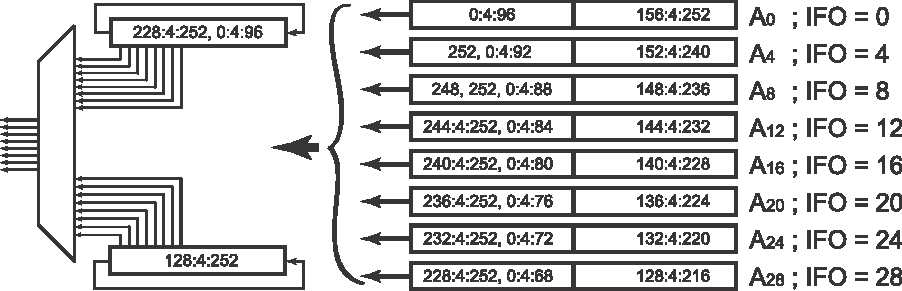
\includegraphics [width=1\columnwidth] {figures/Pilots.pdf} }
	\caption{Circuit for the known-pilots shift register.}
	\label{fig:Pilots}
\end{figure}
%Due to the 4 sample offset between consecutive pilots used for computation, four-fold resource sharing can naturally be performed at the same clock rate for computation of $V_{i}$.

Multiply accumulate blocks are shared for computing four sequential $V_{\tilde{\epsilon}}$ values over four successive clock periods. Fig.~\ref{fig:subsampling} demonstrates how this is done. $P_k$ is received in every clock cycle. $P_{4k}$ is the subsampling of $P_k$, taking a subset of the most significant bits from $P_k$ every four cycles. The cross-correlation is performed with the values of $P_{4k}$. Two multipliers, \emph{M1} and \emph{M2} are used to compute the values of 8 cross-correlations $V_{\tilde{\epsilon}}$ in parallel. Each multiplier performs multiplications sequentially between $P_{4k}$ and the corresponding transmitted pilots in 4 sets of $A_{\tilde{\epsilon}}$. The products are accumulated to the values of $V_{\tilde{\epsilon}}$. When all pilots are computed, the maximum operation, $argmax|V|$, is performed on 8 $V_{\tilde{\epsilon}}$ values to estimate the IFO.

\begin{figure}
	\centerline{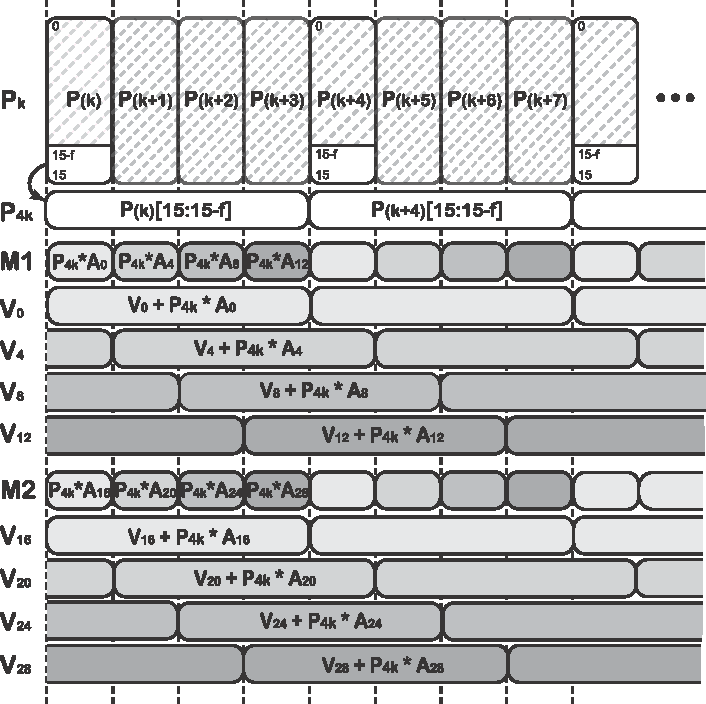
\includegraphics [width=1\columnwidth] {figures/Subsampling.pdf} }
	\caption{Resource sharing approach for computing $V_{\tilde{\epsilon}}$.}
	\label{fig:subsampling}
\end{figure}


\begin{figure}
	\centerline{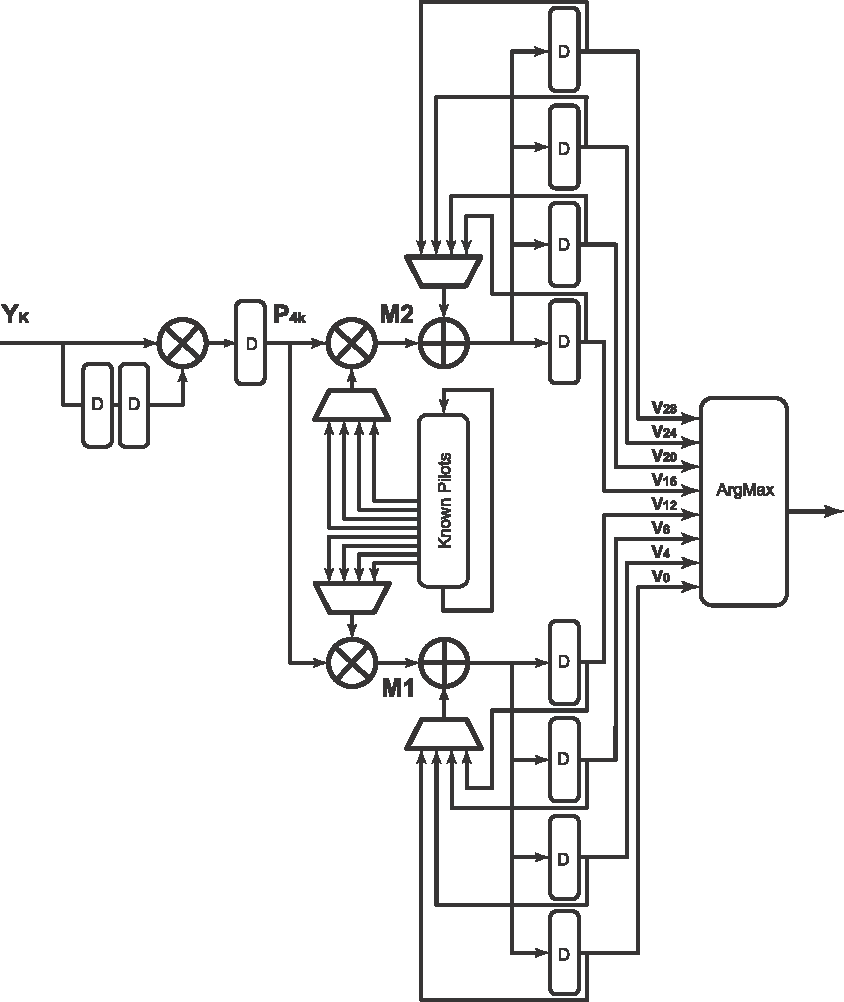
\includegraphics [width=0.95\columnwidth] {figures/ProposedStruc2.pdf} }
	\caption{Architecture of proposed IFO estimator.}
	\label{fig:ProposedStruc}
\end{figure}

To design an optimised architecture for IFO estimation, the multiply-add formula of $V_{\tilde{\epsilon}}$ is mathematically manipulated into what is effectively a multiply-accumulate form.
When one received sample is taken, $V_{\tilde{\epsilon}}$ can be expressed in the form of accumulations as in
\begin{eqnarray}
\label{complexVi}
V_{\tilde{\epsilon}}(n)	&=&   A_{\tilde{\epsilon}}(n) P(n)  + V_{\tilde{\epsilon}}(n-1), \nonumber \\
	 %&=&  (\Re{\{R\}}+i \Im{\{R\}}) (\Re{\{P_i\}} - i \Im{\{P_i\} }) \nonumber\\
	%&  &   + (\Re{\{Acc\}}+i \Im{\{Acc\}}),
						&=& (\Re{\{C_A\}} - i \Im{\{C_A\}})  (\Re{\{P(n)\}} + i \Im{\{P(n)\}}) \nonumber \\
	 					&  &+ (\Re{\{V_{\tilde{\epsilon}}(n-1)\}}+i \Im{\{V_{\tilde{\epsilon}}(n-1)\}})
\end{eqnarray}
where $\Re{\{.\}}$ and $\Im{\{.\}}$ denote the real and imaginary parts, respectively, and \emph{P(n)}, $A_{\tilde{\epsilon}}(n)$ denote the current values of the correlation of two consecutive received pilots and corresponding transmitted pilots, respectively.
$V_{\tilde{\epsilon}}(n-1)$ is the accumulated value of $V_{\tilde{\epsilon}}$.
To employ multiplierless correlation, $A_{\tilde{\epsilon}}$ are normalized to values $C_A$ whose real and imaginary parts have values in \{-1, 0, 1\}, and the wordlength of \emph{P(n)} and $V_{\tilde{\epsilon}}$ in fixed point format can be adjusted to increase estimation accuracy at the cost of increased hardware resource consumption.
The real and imaginary parts of $V_{\tilde{\epsilon}}$ can then be computed as
\begin{eqnarray}
\label{realimaginaryVi}
\Re{\{V_{\tilde{\epsilon}}(n)\}} &=& \Re{\{C_A\}} \Re{\{ P(n)\}}+\Im{\{C_A\}} \Im{\{ P(n)\}} \nonumber \\
								& &+ \Re{\{V_{\tilde{\epsilon}}(n-1)\}} , 					\nonumber \\
\Im{\{V_{\tilde{\epsilon}}(n)\}} &=& \Re{\{C_A\}} \Im{\{ P(n)\}}-\Im{\{C_A\}} \Re{\{ P(n)\}}	\nonumber \\
								& &+ \Im{\{V_{\tilde{\epsilon}}(n-1)\}}
\end{eqnarray}

The proposed resource sharing architecture for the IFO estimator is shown in Fig.~\ref{fig:ProposedStruc}. The \emph{ArgMax} module finds the maximum of the 8 $V_{\tilde{\epsilon}}$ values in order to identify the corresponding IFO estimate.
The novelty of this IFO estimator is in terms of algorithmic improvements and architecture optimisation. This is achieved by firstly reformulating the equation into an expression that is computable with efficient shared resource circuitry.
Thanks to the significant hardware reduction achieved, this IFO estimator can be feasibly implemented on a low-power, limited hardware resource FPGA, while simultaneously ensuring that performance is maintained by a trade off between number of pilots against word length.

We are able to demonstrate that the algorithm and structure optimisations mentioned above retain competitive estimation accuracy compared to conventional approaches, while also offering significant reductions in hardware resource usage.
This makes it possible to implement a high-performance OFDM receiver on a low-power FPGA, especially where the available number of DSP blocks is limited.

\subsection{Simulation}
\label{sec:Sim}
Many variants of the proposed method were simulated in MATLAB using different channel models and the parameter set of the IEEE~802.16-2009 downlink preamble. Performance of the implementation was compared to the theoretical performance of some state of the art methods.
This was assessed primarily in terms of the probability of failed estimation (POFE) with respect to channel SNR.
POFE, which is widely used to evaluate the performance of IFO estimation~\cite{Park2002,Shim2006,Morelli2008}, measures the number of fail estimations divided by the total number of IFO estimations.
Overall, 100,000 IFO estimations were simulated in AWGN and Stanford University Interim (SUI)~\cite{V.ErcegJuly2003} frequency selective channels.
IFO estimation is performed with non-ideal FFO compensation, and FFO is determined and compensated using the method of Kim and Park~\cite{Kim2008}.
The simulation also verifies the performance of the proposed method under the effect of RTO caused by imperfect STO estimation (assuming that STO estimation is still within the CP and does not cause ISI).
In addition, a randomly generated amount of STO is added in the range from 0 to $N_{CP}-L-1$, where \emph{L} is the length of CIR.

We first investigate the performance degradation compared to theoretical performance as a result of reducing the number of pilots as proposed. Next, we will investigate the effect of wordlength optimisation.
In both cases, comparisons are made with established methods in the literature that can be simulated but are otherwise infeasible for hardware implementation, namely the conventional method in \cite{Park2002} (\emph{PCH}) that is applied to one training block with 100 pilots.
In addition,  two state of the art methods are also simulated for comparison.
Firstly, metric \emph{SY} from \cite{Shim2006} as defined by,

\begin{eqnarray}
\label{equ:SY}
\hat{\epsilon} &=&\underset{\tilde{\epsilon} \in S_{IFO}}{\operatorname{argmax}} \left| \mu_{_{SY}}(\tilde{\epsilon})  \right|,	 \nonumber \\
\mu_{_{SY}}(\tilde{\epsilon}) &=& \Re{\left\{\sum_{k=1}^{\frac{N}{2}} Y^{*}_{(2k-2)} Y_{(2k)}  X^{*}_{(2k-\tilde{\epsilon})} X_{(2k-2-\tilde{\epsilon})}\right\}}
\end{eqnarray}
Secondly, metric \emph{MM} from \cite{Morelli2008},

%\todo[inline]{**Thinh -  the equation above doesn't include  $\hat{\epsilon}$ and is very similar to the next equation -- is there some problem? (ivm)}
\begin{eqnarray}
\label{equ:MM}
\hat{\epsilon} &=& \underset{\tilde{\epsilon} \in S_{IFO}}{\operatorname{argmax}} \left| \mu_{_{MM}}(\tilde{\epsilon}) \right|,	 \nonumber \\
\mu_{_{MM}}(\tilde{\epsilon}) &=& \Re{\left\{e^{i\frac{\pi}{4}} \sum_{k=1}^{\frac{N}{2}} Y^{*}_{(2k-2)} Y_{(2k)}  X^{*}_{(2k-\tilde{\epsilon})}  X_{(2k-2-\tilde{\epsilon})}\right\}}
\end{eqnarray}
where $\Re{\{.\}}$ denotes the real part.

We are unaware of any published circuits for these methods, because of their complex computation. The very large hardware requirement for these respective metrics does not lend either method to feasible implementation on a low cost, low power FPGA (unlike the proposed method).

\subsubsection{Performance Comparison}

The performance of the proposed method, denoted \emph{Prop}, is evaluated in comparison to the theoretical performance of state of the art methods by Park et. al.~\cite{Park2002}, Shim and You~\cite{Shim2006} and Morelli and Moretti~\cite{Morelli2008}, denoted \emph{PCH}, \emph{SY} and \emph{MM}, respectively in the previous subsection.
The theoretical performance is computed with full precision using full multiplication.
However, it must be noted that implementing this directly in hardware would be prohibitive due to the large number of multiplication operations needed.
In fact, hardware implementation would conventionally use sign-bit correlation instead of full precision correlation, as mentioned previously. Thus the full multiplication results shown here are undoubtedly better than those achievable in practice, and thus can be considered as upper performance bounds.
For more realistic data, we also provide results from sign-bit correlation versions of the above, denoted
\emph{PCH\_sb}, \emph{SY\_sb}, and \emph{MM\_sb} respectively.

The proposed method, evaluated against these, uses 50 spread pilots with indices that are multiples of 4.
For the sake of comparison, an additional implementation of \emph{PCH} is reported which, like the proposed method, uses only 50 pilots, but which are placed continuously rather than being spread. This is denoted \emph{PCH\_50}.
Figs.~\ref{fig:IFO_AWGN} and \ref{fig:IFO_AWGN_RTO} plot performance results for all methods in an AWGN channel, with and without RTO respectively, and reveal that the proposed method generally performs well, especially at higher SNRs. Considering more realistic channel models, Figs.~\ref{fig:IFO_SUI1} and \ref{fig:IFO_SUI2} plot the performance of all methods in SUI1, and SUI2 channels respectively, and similarly show that the proposed method performs well, especially at higher SNRs.


\begin{figure}
	\centering
	\begin{tikzpicture}
	\begin{semilogyaxis}[ xlabel=SNR(dB), ylabel=Probability of Fail Estimation (\%), legend columns=4,	legend style={at={(0.5,1.02)}, anchor=south, cells={anchor=west}, draw=none},
						 xmax=12, ymin=0.001, ymax=100, x post scale=1.4]
		\addplot+[black, style={dashed},every mark/.append style={mark=square, style=solid}] 		 table [x index=0, y index=1] {./Dat/AWGN_cmp_meth.dat};
		\addlegendentry{MM};
		\addplot+[black, style={dotted},	every mark/.append style={mark=square, style=solid}]		 table [x index=0, y index=2] {./Dat/AWGN_cmp_meth.dat};
		\addlegendentry{MM\_sb};
		\addplot+[black, style={dashed},	every mark/.append style={mark=diamond, style=solid}]	 table [x index=0, y index=3] {./Dat/AWGN_cmp_meth.dat};
		\addlegendentry{SY};
		\addplot+[black, style={dotted},	every mark/.append style={mark=diamond, style=solid}]	 table [x index=0, y index=4] {./Dat/AWGN_cmp_meth.dat};
		\addlegendentry{SY\_sb};
		\addplot+[black, style={dashed},	every mark/.append style={mark=triangle, style=solid}] 	 table [x index=0, y index=5] {./Dat/AWGN_cmp_meth.dat};
		\addlegendentry{PCH};
		\addplot+[black, style={dotted},	every mark/.append style={mark=triangle, style=solid}]	 table [x index=0, y index=6] {./Dat/AWGN_cmp_meth.dat};
		\addlegendentry{PCH\_sb};
		\addplot+[black, style={solid},	every mark/.append style={mark=o, style=solid}]			 table [x index=0, y index=7] {./Dat/AWGN_cmp_meth.dat};
		\addlegendentry{PCH\_50};
		\addplot+[black, style={solid},	every mark/.append style={mark=*, style=solid}]			 table [x index=0, y index=8] {./Dat/AWGN_cmp_meth.dat};
		\addlegendentry{Prop};
	\end{semilogyaxis}
	\end{tikzpicture}
\caption{Fail rate of IFO estimation methods in AWGN channel without RTO.}
\label{fig:IFO_AWGN}
\end{figure}

% add new figure for IFO estimation with RTO
\begin{figure}
	\centering
	\begin{tikzpicture}
	\begin{semilogyaxis}[ xlabel=SNR(dB), ylabel=Probability of Fail Estimation (\%), legend columns=4,	legend style={at={(0.5,1.02)}, anchor=south, cells={anchor=west}, draw=none},
						 xmax=12, ymin=0.001, ymax=100, x post scale=1.4]
		\addplot+[black, style={dashed},every mark/.append style={mark=square, style=solid}] 		 table [x index=0, y index=1] {./Dat/AWGN_cmp_meth_toff.dat};
		\addlegendentry{MM};
		\addplot+[black, style={dotted},	every mark/.append style={mark=square, style=solid}]		 table [x index=0, y index=2] {./Dat/AWGN_cmp_meth_toff.dat};
		\addlegendentry{MM\_sb};
		\addplot+[black, style={dashed},	every mark/.append style={mark=diamond, style=solid}]	 table [x index=0, y index=3] {./Dat/AWGN_cmp_meth_toff.dat};
		\addlegendentry{SY};
		\addplot+[black, style={dotted},	every mark/.append style={mark=diamond, style=solid}]	 table [x index=0, y index=4] {./Dat/AWGN_cmp_meth_toff.dat};
		\addlegendentry{SY\_sb};
		\addplot+[black, style={dashed},	every mark/.append style={mark=triangle, style=solid}] 	 table [x index=0, y index=5] {./Dat/AWGN_cmp_meth_toff.dat};
		\addlegendentry{PCH};
		\addplot+[black, style={dotted},	every mark/.append style={mark=triangle, style=solid}]	 table [x index=0, y index=6] {./Dat/AWGN_cmp_meth_toff.dat};
		\addlegendentry{PCH\_sb};
		\addplot+[black, style={solid},	every mark/.append style={mark=o, style=solid}]			 table [x index=0, y index=7] {./Dat/AWGN_cmp_meth_toff.dat};
		\addlegendentry{PCH\_50};
		\addplot+[black, style={solid},	every mark/.append style={mark=*, style=solid}]			 table [x index=0, y index=8] {./Dat/AWGN_cmp_meth_toff.dat};
		\addlegendentry{Prop};
	\end{semilogyaxis}
	\end{tikzpicture}
\caption{Fail rate of IFO estimation methods in AWGN channel with RTO.}
\label{fig:IFO_AWGN_RTO}
\end{figure}
%==

\begin{figure}
	\centering
	\begin{tikzpicture}
	\begin{semilogyaxis}[ xlabel=SNR(dB), ylabel=Probability of Fail Estimation (\%), legend columns=4,	legend style={at={(0.5,1.02)}, anchor=south, cells={anchor=west}, draw=none},
						 xmax=12, ymin=0.001, ymax=100, x post scale=1.4]
		\addplot+[black, style={dashed},every mark/.append style={mark=square, style=solid}] 		 table [x index=0, y index=1] {./Dat/SUI1_cmp_meth.dat};
		\addlegendentry{MM};
		\addplot+[black, style={dotted},	every mark/.append style={mark=square, style=solid}]		 table [x index=0, y index=2] {./Dat/SUI1_cmp_meth.dat};
		\addlegendentry{MM\_sb};
		\addplot+[black, style={dashed},	every mark/.append style={mark=diamond, style=solid}]	 table [x index=0, y index=3] {./Dat/SUI1_cmp_meth.dat};
		\addlegendentry{SY};
		\addplot+[black, style={dotted},	every mark/.append style={mark=diamond, style=solid}]	 table [x index=0, y index=4] {./Dat/SUI1_cmp_meth.dat};
		\addlegendentry{SY\_sb};
		\addplot+[black, style={dashed},	every mark/.append style={mark=triangle, style=solid}] 	 table [x index=0, y index=5] {./Dat/SUI1_cmp_meth.dat};
		\addlegendentry{PCH};
		\addplot+[black, style={dotted},	every mark/.append style={mark=triangle, style=solid}]	 table [x index=0, y index=6] {./Dat/SUI1_cmp_meth.dat};
		\addlegendentry{PCH\_sb};
		\addplot+[black, style={solid},	every mark/.append style={mark=o, style=solid}]			 table [x index=0, y index=7] {./Dat/SUI1_cmp_meth.dat};
		\addlegendentry{PCH\_50};
		\addplot+[black, style={solid},	every mark/.append style={mark=*, style=solid}]			 table [x index=0, y index=8] {./Dat/SUI1_cmp_meth.dat};
		\addlegendentry{Prop};
	\end{semilogyaxis}
	\end{tikzpicture}
\caption{Fail rate of IFO estimation methods in SUI1 channel.}
\label{fig:IFO_SUI1}
\end{figure}

\begin{figure}
	\centering
	\begin{tikzpicture}
	\begin{semilogyaxis}[ xlabel=SNR(dB), ylabel=Probability of Fail Estimation (\%), legend columns=4,	legend style={at={(0.5,1.02)}, anchor=south, cells={anchor=west}, draw=none},
						 xmax=12, ymin=0.001, ymax=100, x post scale=1.4]
		\addplot+[black, style={dashed},every mark/.append style={mark=square, style=solid}] 		 table [x index=0, y index=1] {./Dat/SUI2_cmp_meth.dat};
		\addlegendentry{MM};
		\addplot+[black, style={dotted},	every mark/.append style={mark=square, style=solid}]		 table [x index=0, y index=2] {./Dat/SUI2_cmp_meth.dat};
		\addlegendentry{MM\_sb};
		\addplot+[black, style={dashed},	every mark/.append style={mark=diamond, style=solid}]	 table [x index=0, y index=3] {./Dat/SUI2_cmp_meth.dat};
		\addlegendentry{SY};
		\addplot+[black, style={dotted},	every mark/.append style={mark=diamond, style=solid}]	 table [x index=0, y index=4] {./Dat/SUI2_cmp_meth.dat};
		\addlegendentry{SY\_sb};
		\addplot+[black, style={dashed},	every mark/.append style={mark=triangle, style=solid}] 	 table [x index=0, y index=5] {./Dat/SUI2_cmp_meth.dat};
		\addlegendentry{PCH};
		\addplot+[black, style={dotted},	every mark/.append style={mark=triangle, style=solid}]	 table [x index=0, y index=6] {./Dat/SUI2_cmp_meth.dat};
		\addlegendentry{PCH\_sb};
		\addplot+[black, style={solid},	every mark/.append style={mark=o, style=solid}]			 table [x index=0, y index=7] {./Dat/SUI2_cmp_meth.dat};
		\addlegendentry{PCH\_50};
		\addplot+[black, style={solid},	every mark/.append style={mark=*, style=solid}]			 table [x index=0, y index=8] {./Dat/SUI2_cmp_meth.dat};
		\addlegendentry{Prop};
	\end{semilogyaxis}
	\end{tikzpicture}
\caption{Fail rate of IFO estimation methods in SUI2 channel.}
\label{fig:IFO_SUI2}
\end{figure}

Under these experimental conditions, \emph{PCH} and \emph{SY} achieve equivalent performance in AWGN without RTO and in SUI1 channels.
However, \emph{SY} degrades more drastically than \emph{PCH} in the SUI2 channel at SNRs above 1\,dB.
\emph{SY} also deteriorates in the case of AWGN with RTO. This method appears to be very sensitive to large RTO, while \emph{MM} and \emph{PCH} exhibit better robustness to RTO.
The accuracy of \emph{MM} is slightly lower than that of \emph{PCH} at SNRs below 0\,dB, while performance is very similar at larger SNRs.
Also note the performance of the conventional approach implementations, \emph{PCH\_sb}, \emph{SY\_sb}, \emph{MM\_sb} which degrade significantly with SNR, especially in the SUI1, SUI2 channels.

Apart from at very low SNRs, the proposed method, \emph{Prop}, achieves almost identical performance to the simulated upper bound \emph{PCH}, even in the presence of RTO.
It should be noted that \emph{Prop} achieves this while allowing the use of resource sharing through sparse pilot computation. This will be used below to achieve a significant hardware saving.
According to simulation results, \emph{Prop}, with its spread pilots, is also more accurate than \emph{PCH\_50} that uses the same number of pilots, but places them continuously.

\subsubsection{Wordlength Optimisation}
Since sign-bit correlation degrades IFO estimation performance, specially in frequency selective channels, the proposed method instead employs multiplierless correlation to improve accuracy and robustness.
The complexity of this approach is dependent on the wordlength chosen for the correlation computation.
We now investigate how wordlength affects the performance of the proposed implementation, again compared to the theoretical bound, \emph{PCH}, as well as to the performance of a conventional sign-bit implementation, \emph{PCH\_sb}.
We denote wordlength using the notation $Q1.f$, meaning a single integer bit and $f$ fractional bits.
Evaluations are performed for $f$ of 1, 2, 7, and 15 bits. These results will be plotted in the following figures with the labels \emph{Prop\_1b}, \emph{Prop\_2b}, \emph{Prop\_7b}, and \emph{Prop\_15b}, respectively.
Figs.~\ref{fig:IFO_Qb_AWGN} and \ref{fig:IFO_Qb_AWGN_RTO} plot the performance in AWGN (with and without RTO), with all tested wordlengths in the proposed method performing comparably to \emph{PCH} (and being much better than \emph{PCH\_sb} at SNRs exceeding about 2\,dB).
Figs.~\ref{fig:IFO_Qb_SUI1} and \ref{fig:IFO_Qb_SUI2} plot the results when using the more realistic SUI1 and SUI2 channel models.

\begin{figure}
	\centering
	\begin{tikzpicture}
	\begin{semilogyaxis}[ xlabel=SNR(dB), ylabel=Probability of Fail Estimation (\%), legend columns=3,	legend style={at={(0.5,1.02)}, anchor=south, cells={anchor=west}, draw=none},
						 xmax=12, ymin=0.001, ymax=100, x post scale=1.4]
		\addplot+[black, style={dashed},	every mark/.append style={mark=triangle, style=solid}] 	 table [x index=0, y index=1] {./Dat/AWGN_Qb.dat};
		\addlegendentry{PCH};
		\addplot+[black, style={dotted},	every mark/.append style={mark=triangle, style=solid}]	 table [x index=0, y index=2] {./Dat/AWGN_Qb.dat};
		\addlegendentry{PCH\_sb};
		\addplot+[black, style={dashed}, every mark/.append style={mark=square, style=solid}] 	 table [x index=0, y index=3] {./Dat/AWGN_Qb.dat};
		\addlegendentry{Prop\_15b};
		\addplot+[black, style={dashed},	every mark/.append style={mark=diamond, style=solid}]	 table [x index=0, y index=4] {./Dat/AWGN_Qb.dat};
		\addlegendentry{Prop\_7b};
		\addplot+[black, style={solid},	every mark/.append style={mark=*, style=solid}]			 table [x index=0, y index=5] {./Dat/AWGN_Qb.dat};
		\addlegendentry{Prop\_2b};
		\addplot+[black, style={dashed},	every mark/.append style={mark=o, style=solid}]			 table [x index=0, y index=6] {./Dat/AWGN_Qb.dat};
		\addlegendentry{Prop\_1b};
	\end{semilogyaxis}
	\end{tikzpicture}
\caption{Fail rate for different wordlengths in AWGN channel without RTO.}
\label{fig:IFO_Qb_AWGN}
\end{figure}

\begin{figure}
\centering
	\begin{tikzpicture}
	\begin{semilogyaxis}[ xlabel=SNR(dB), ylabel=Probability of Fail Estimation (\%), legend columns=3,	legend style={at={(0.5,1.02)}, anchor=south, cells={anchor=west}, draw=none},
						 xmax=12, ymin=0.001, ymax=100, x post scale=1.4]
		\addplot+[black, style={dashed},	every mark/.append style={mark=triangle, style=solid}] 	 table [x index=0, y index=1] {./Dat/AWGN_Qb_toff.dat};
		\addlegendentry{PCH};
		\addplot+[black, style={dotted},	every mark/.append style={mark=triangle, style=solid}]	 table [x index=0, y index=2] {./Dat/AWGN_Qb_toff.dat};
		\addlegendentry{PCH\_sb};
		\addplot+[black, style={dashed}, every mark/.append style={mark=square, style=solid}] 	 table [x index=0, y index=3] {./Dat/AWGN_Qb_toff.dat};
		\addlegendentry{Prop\_15b};
		\addplot+[black, style={dashed},	every mark/.append style={mark=diamond, style=solid}]	 table [x index=0, y index=4] {./Dat/AWGN_Qb_toff.dat};
		\addlegendentry{Prop\_7b};
		\addplot+[black, style={solid},	every mark/.append style={mark=*, style=solid}]			 table [x index=0, y index=5] {./Dat/AWGN_Qb_toff.dat};
		\addlegendentry{Prop\_2b};
		\addplot+[black, style={dashed},	every mark/.append style={mark=o, style=solid}]			 table [x index=0, y index=6] {./Dat/AWGN_Qb_toff.dat};
		\addlegendentry{Prop\_1b};
	\end{semilogyaxis}
	\end{tikzpicture}
\caption{Fail rate for different wordlengths in AWGN channel with RTO.}
\label{fig:IFO_Qb_AWGN_RTO}
\end{figure}

\begin{figure}
\centering
	\begin{tikzpicture}
	\begin{semilogyaxis}[ xlabel=SNR(dB), ylabel=Probability of Fail Estimation (\%), legend columns=3,	legend style={at={(0.5,1.02)}, anchor=south, cells={anchor=west}, draw=none},
						 xmax=12, ymin=0.001, ymax=100, x post scale=1.4]
		\addplot+[black, style={dashed},	every mark/.append style={mark=triangle, style=solid}] 	 table [x index=0, y index=1] {./Dat/SUI1_Qb.dat};
		\addlegendentry{PCH};
		\addplot+[black, style={dotted},	every mark/.append style={mark=triangle, style=solid}]	 table [x index=0, y index=2] {./Dat/SUI1_Qb.dat};
		\addlegendentry{PCH\_sb};
		\addplot+[black, style={dashed}, every mark/.append style={mark=square, style=solid}] 	 table [x index=0, y index=3] {./Dat/SUI1_Qb.dat};
		\addlegendentry{Prop\_15b};
		\addplot+[black, style={dashed},	every mark/.append style={mark=diamond, style=solid}]	 table [x index=0, y index=4] {./Dat/SUI1_Qb.dat};
		\addlegendentry{Prop\_7b};
		\addplot+[black, style={solid},	every mark/.append style={mark=*, style=solid}]			 table [x index=0, y index=5] {./Dat/SUI1_Qb.dat};
		\addlegendentry{Prop\_2b};
		\addplot+[black, style={dashed},	every mark/.append style={mark=o, style=solid}]			 table [x index=0, y index=6] {./Dat/SUI1_Qb.dat};
		\addlegendentry{Prop\_1b};
	\end{semilogyaxis}
	\end{tikzpicture}
\caption{Fail rate for different wordlengths in SUI1 channel.}
\label{fig:IFO_Qb_SUI1}
\end{figure}

\begin{figure}
\centering
	\begin{tikzpicture}
	\begin{semilogyaxis}[ xlabel=SNR(dB), ylabel=Probability of Fail Estimation (\%), legend columns=3,	legend style={at={(0.5,1.02)}, anchor=south, cells={anchor=west}, draw=none},
						 xmax=12, ymin=0.001, ymax=100, x post scale=1.4]
		\addplot+[black, style={dashed},	every mark/.append style={mark=triangle, style=solid}] 	 table [x index=0, y index=1] {./Dat/SUI2_Qb.dat};
		\addlegendentry{PCH};
		\addplot+[black, style={dotted},	every mark/.append style={mark=triangle, style=solid}]	 table [x index=0, y index=2] {./Dat/SUI2_Qb.dat};
		\addlegendentry{PCH\_sb};
		\addplot+[black, style={dashed}, every mark/.append style={mark=square, style=solid}] 	 table [x index=0, y index=3] {./Dat/SUI2_Qb.dat};
		\addlegendentry{Prop\_15b};
		\addplot+[black, style={dashed},	every mark/.append style={mark=diamond, style=solid}]	 table [x index=0, y index=4] {./Dat/SUI2_Qb.dat};
		\addlegendentry{Prop\_7b};
		\addplot+[black, style={solid},	every mark/.append style={mark=*, style=solid}]			 table [x index=0, y index=5] {./Dat/SUI2_Qb.dat};
		\addlegendentry{Prop\_2b};
		\addplot+[black, style={dashed},	every mark/.append style={mark=o, style=solid}]			 table [x index=0, y index=6] {./Dat/SUI2_Qb.dat};
		\addlegendentry{Prop\_1b};
	\end{semilogyaxis}
	\end{tikzpicture}
\caption{Fail rate for different wordlengths in SUI2 channel.}
\label{fig:IFO_Qb_SUI2}
\end{figure}

It can be seen from the plots that each of the tested wordlengths achieves much better performance and exhibits greater robustness to frequency selective channels than the sign-bit realisation of the conventional approach, \emph{PCH\_sb}.
Additionally, these realisations of the proposed method do not suffer as much degradation in the presence of RTO.
Moreover, it is possible to improve low SNR performance by adopting a longer wordlength with the proposed method, at a cost of increased hardware complexity. Increasing wordlength does improve results slightly, with the step from 1 to 2 bits being the most significant gain. By contrast, increasing from 2 to 7 or from 7 to 15 bits has little impact.
In general, \emph{Prop\_2b} achieves an estimation accuracy close to that of the theoretical performance bound, \emph{PCH}, at intermediate and higher SNRs, even though it involves computation with fewer bits, and can hence be implemented more efficiently.

%---------------------------------------------------------------------------------------------------------------------------------------------------------------------
\subsection{FPGA Implementation}
\label{sec:Imple}
The analysis in Section~\ref{sec:Sim} suggests that the proposed method offers comparable estimation performance to existing methods in the literature.
As a result of the simplifications inherent in the proposed approach, this should be achievable at a reduced hardware cost.
This section now quantifies this hardware cost, for an FPGA-based implementation.
It is important to note that these hardware savings are accessible for a number of target implementation devices, although we are interested primarily in FPGA implementation as part of our work on leveraging FPGA reconfigurability in cognitive radios.

\subsubsection{Conventional Approach}
To obtain the theoretical performance previously discussed in Section \ref{sec:Sim} and denoted as \emph{PCH}, the computation of the estimation metric in \cite{Park2002}, using 100 pilots, would require about 200 complex multipliers, resulting in the use of over 600 DSP blocks. This may exceed the available resources on small devices, or leave insufficient resources for other tasks on larger devices.
As the number of multiplications required for a full implementation of the approach is prohibitive, the conventional approach for implementation, as we have discussed, uses sign-bit correlation~\cite{Kim2008}.
This conventional implementation uses all 100 pilots in the long preamble to perform sign-bit correlation, and multiply\_adds are eliminated at taps where the pilots of the long preamble are not used.
This implementation mirrors the \emph{PCH\_sb} in Section \ref{sec:Sim}, and allows us to quantify the benefits of our proposed approach against a known reference benchmark.

\subsubsection{Proposed Approach}

The proposed architecture for the IFO estimator, implemented with several different wordlengths of $P(n)$ and $V_{\tilde{\epsilon}}$ in (\ref{complexVi}), are compared to allow us to explore the hardware costs associated with the respective implementations.
Four fixed point formats for $P(n)$, are investigated: Q1.1, Q1.2, Q1.7, and Q1.15.
$V_{\tilde{\epsilon}}$  is represented accordingly in Q7.1, Q7.2, Q7.7, and Q7.15 formats to avoid overflow.

In order to obtain a comprehensive optimised implementation, these circuits are each implemented using two different structures.
The first uses only logic elements (LE) for computation, while the second uses Xilinx DSP48A1 \cite{ug389} primitives.
Considering (\ref{realimaginaryVi}), $\Re{\{V_{\tilde{\epsilon}}(n)\}}, \Im{\{V_{\tilde{\epsilon}}(n)\}}$ can be computed effectively using two DSP blocks as 3-input adders, instead of 4 blocks as would be usual.
Fig.~\ref{fig:DSP48Acc} illustrates how this is done for $\Re{\{V_{\tilde{\epsilon}}(n)\}}$, and similarly for $\Im{\{V_{\tilde{\epsilon}}(n)\}}$.
\begin{figure}
	\centerline{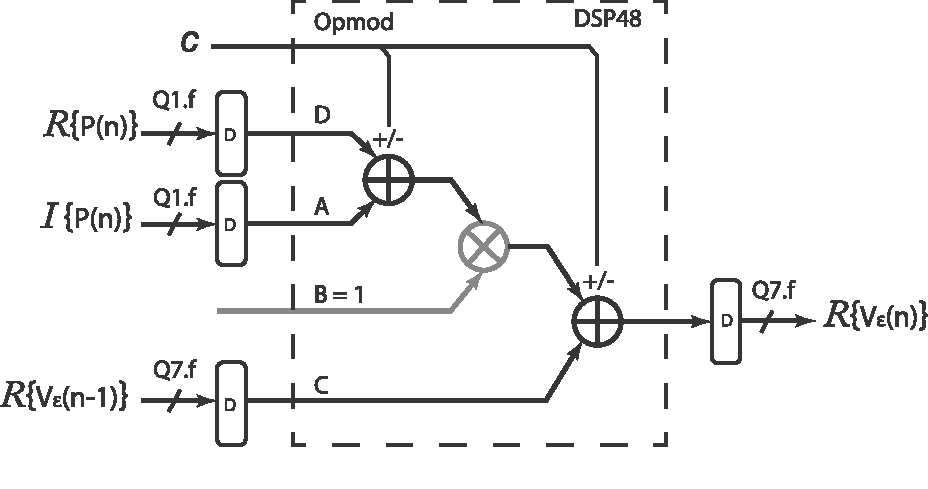
\includegraphics [width=1\columnwidth] {figures/DSP48Acc.pdf} }
	\caption{DSP block based 3-input adder for correlation.}
	\label{fig:DSP48Acc}
\end{figure}
Note that the solution presented in Fig.~\ref{fig:DSP48Acc} is optimised for QPSK modulated pilots (since their amplitudes are identical) as specified in IEEE~802.16, as well as in most OFDM-based standards.
The normalisation performed in (\ref{realimaginaryVi}) allows the correlation to be reduced to two DSP blocks operating as 3-input adders (instead of 4 DSP blocks with multipliers as would be usual).
These methods correspond to \emph{Prop\_1b}, \emph{Prop\_2b}, \emph{Prop\_7b}, and \emph{Prop\_15b} that were investigated for estimation accuracy in Section~\ref{sec:Sim}.

\subsection{Implementation Results}
The circuits were synthesised and fully implemented using Xilinx ISE 13.2, targeting the low-power Xilinx Spartan-6 XC6SLX75T FPGA.
The results are reported in terms of the number of flip-flops (FF), look-up tables (LUT), and DSP48 blocks, along with dynamic power consumption, as summarised in Table~\ref{tab:Imp_Rpt}.
\begin{table}[h]
	\centering
	\caption{Resource utilisation and dynamic power consumption of IFO estimators.}
	\label{tab:Imp_Rpt}
	\renewcommand{\arraystretch}{1.2}

	\begin{tabular}{r|r|r|r|r|r}

       \hline \hline
    		  \makebox[1.1cm][c]{IFO est. Cir.} 	& \#FF & \#LUT  & \#DSP & Fre (MHz) & D. Power \\
    	\hline
		\textbf{conv\_100p}		& 3270 (3\%)	& 1837 (3\%)	& 3 &  142 	&  42	mW \\
		Prop\_1b\_LE			& 328 (1\%)		& 370 (1\%)		& 3 &  136 	&  9		mW\\
		\textbf{Prop\_2b\_LE}	& 350 (1\%)		& 390 (1\%)		& 3 &  136 	&  10 	mW\\
		Prop\_7b\_LE			& 460 (1\%)		& 471 (1\%)		& 3 &  136 	&  12 	mW\\
		Prop\_15b\_LE		      & 735 (1\%)		& 696 (1\%)		& 3 &  134 	&  17 	mW\\

		Prop\_1b\_DSP			& 328 (1\%)		& 306 (1\%)		& 7 &  78   	&  11 	mW\\
		Prop\_2b\_DSP			& 350 (1\%)		& 319 (1\%)		& 7 &  78   	&  12	mW\\
		Prop\_7b\_DSP			& 460 (1\%)		& 379 (1\%)		& 7 &  77   	&  14	mW\\
		Prop\_15b\_DSP			& 735 (1\%)		& 591 (1\%)		& 7 &  77 	&  18 	mW\\
    	\hline \hline
    \end{tabular}
\end{table}

%\todo[inline]{**Thinh: the table above (table 5.1) has some corrupted row titles - you should either increase the row widths or remove all the width specifiers. (ivm)}

\emph{conv\_100p} refers to the conventional approach, implemented using sign-bit correlation over 100 pilots.
\emph{Prop\_fb\_LE}, \emph{Prop\_fb\_DSP}, in which $f$ = 1, 2, 7 and 15 (corresponding to received sample format Q1.$f$), denote the circuits of corresponding wordlengths, implemented using logic elements and DSP48 blocks, respectively.
Referring to the table, the proposed implementation shows that significant improvement in resource usage and dynamic power consumption is possible with the proposed method.

The hardware resources used by \emph{Prop\_fb\_LE} and \emph{Prop\_fb\_DSP} increase gradually, in terms of FFs and LUTs, as the wordlength increases.
The number of FFs used in \emph{Prop\_fb\_DSP} and \emph{Prop\_fb\_LE} is equal, while \emph{Prop\_fb\_DSP} uses fewer LUTs since the DSP blocks are used for the 3-input additions.

The \emph{Prop\_fb\_LE} implementations use 3 DSP blocks to compute $P(n)$, while \emph{Prop\_fb\_DSP} require an additional 4 DSP blocks to perform the correlation.
\emph{Prop\_fb\_LE}, \emph{Prop\_fb\_DSP} both consume far fewer LUT and FF resources than the conventional \emph{conv\_100p} implementation.

For \emph{Prop\_2b\_LE}, the number of FFs and LUTs is reduced by 90\% and 79\% respectively compared to the conventional \emph{conv\_100p} approach.

The maximum frequencies of circuits, reported after place and route, comfortably exceed the timing requirements for IEEE~802.16 synchronisation whose sampling frequency is below 25~MHz.
A post-place-and-route simulation was used to estimate the power consumption of the system at a clock rate of 50{\thinspace}MHz, using the Xilinx XPower tool -- also shown in table \ref{tab:Imp_Rpt}.

\emph{Prop\_fb\_LE} implementations consume less power than the equivalent \emph{Prop\_fb\_DSP} implementations.
All implementations of the proposed method consume significantly less power than the conventional implementation.
\emph{Prop\_2b\_LE} consumes just 22\% of the power consumed by \emph{conv\_100p}.

In subsection \ref{sec:Sim}, we established that \emph{Prop\_2b\_LE} easily outperforms the conventional approach in terms of estimation accuracy.
In this subsection, we have shown that it does so with a significant hardware resource saving, and with significantly reduced power consumption.
In fact, the estimation performance of \emph{Prop\_2b\_LE}, in AWGN and SUI channels (except at very low SNR), is close to the theoretical bound of \emph{PCH}, which would demand a significant proportion of the FPGAs resources if it were implemented conventionally.
Meanwhile, \emph{Prop\_2b\_LE} is extremely efficient, consuming less than 1\% of the resources available on a low-power Spartan-6 XC6SLX75 FPGA.
Beyond IEEE 802.16-2009, the folded resource sharing architecture, which leverages sub-sample spaced OFDM pilots, can be adopted for use in other OFDM standards (including IEEE 802.11 and IEEE 802.22).

%---------------------------------------------------------------------------------
\section{Summary}
%---------------------------------------------------------------------------------

This chapter investigated IFO estimation in OFDM-based systems such as IEEE 802.16. A technique is proposed for efficient implementation of IFO estimation, which aims in particular for a low power and low resource utilisation.
Since IFO estimation contributes significantly to the complexity of a robust synchroniser design, this work is important for multistandard radios, or applications where significant frequency variation is expected. Robust IFO estimation allows for relaxed analogue RF constraints, leading to reduced cost. A modified timing metric is derived which allows for resource sharing to reduce both resource requirements as well as power consumption. The proposed implementation makes use of a four-fold resource sharing architecture to significantly reduce hardware cost, while multiplierless correlation with optimised wordlength is used to improve estimation accuracy in comparison to a conventional implementation approach using signbit correlation.
The method is shown to perform as well as current state-of-the-art methods that employ multiplier-based correlation, and yet with significantly improved power and resource requirements. Dynamic power consumption is reduced by 78\% over even a sign-bit version of the conventional approach, yet it offers better estimation performance in both AWGN and frequency selective channels.
Beyond IEEE 802.16-2009, the folded resource sharing method, which leverages sub-sample spaced OFDM pilots, can be adopted for use in other OFDM standards (including IEEE 802.11 and IEEE 802.22). Multiplierless correlation with word length optimisation is already used within communication systems, however the trade off between the number of pilots and computational accuracy for timing synchronisation is relatively unexplored in the research literature to date.
